\documentclass[12pt,a4paper]{article}
\usepackage[margin=2.5cm]{geometry}
\usepackage[utf8]{inputenc}
\usepackage[T1]{fontenc}
% babel Indonesian unavailable as .ldf on this TeX Live: set labels manually.
\renewcommand{\contentsname}{Daftar Isi}
\renewcommand{\figurename}{Gambar}
\renewcommand{\tablename}{Tabel}
\renewcommand{\refname}{Referensi}
\usepackage{hyperref}
\usepackage{booktabs}
\usepackage{enumitem}
\usepackage{graphicx}
\usepackage{xcolor}
\usepackage{tikz}
\usetikzlibrary{arrows.meta, positioning}
\hypersetup{colorlinks=true, linkcolor=blue!70!black, urlcolor=blue!70!black,
  pdftitle={SIGAP - Dokumentasi dan Buku Panduan Penggunaan}}

\tikzset{
  alir/.style={rectangle, rounded corners, draw=blue!70!black, fill=blue!5,
    minimum width=4.6cm, minimum height=0.85cm, align=center, font=\footnotesize},
  panah/.style={-{Stealth}, thick, blue!70!black}
}

\begin{document}

% ---------------- Sampul ----------------
\begin{center}
  \vspace*{1.5cm}
  {\Large \textbf{SIGAP}}\\[0.4cm]
  {\large Dokumentasi dan Buku Panduan Penggunaan}\\[0.3cm]
  {\normalsize Sistem Informasi Gerakan Anti Penindasan}\\[1.2cm]
  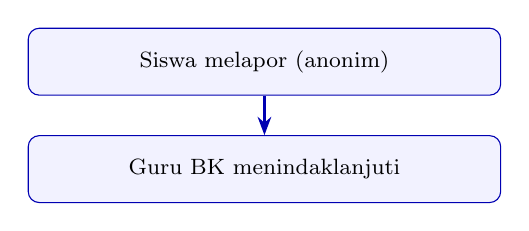
\begin{tikzpicture}
    \node[alir, minimum width=6cm] (a) {Siswa melapor (anonim)};
    \node[alir, minimum width=6cm, below=0.5cm of a] (b) {Guru BK menindaklanjuti};
    \draw[panah] (a) -- (b);
  \end{tikzpicture}\\[1.2cm]
  {\normalsize Versi 1.0 MVP --- 2026}
\end{center}
\clearpage

% ---------------- Isi ----------------
\tableofcontents
\clearpage

\section{Gambaran Aplikasi}
SIGAP (Sistem Informasi Gerakan Anti Penindasan) adalah aplikasi web untuk
pelaporan perundungan (\textit{bullying}) di lingkungan sekolah. Siswa dapat
melapor secara anonim dan memantau status laporannya dengan kode tiket,
sementara Guru BK memverifikasi dan menindaklanjuti setiap laporan yang masuk.

\begin{center}
\begin{tabular}{lll}
\toprule
\textbf{Aktor} & \textbf{Akses} & \textbf{Akun} \\
\midrule
Siswa / Anonim & Isi laporan, cek status tiket & Tidak perlu \\
Guru BK (Admin) & Kelola semua laporan & Username + password \\
\bottomrule
\end{tabular}
\end{center}

\section{Alur Kerja Sistem}
Gambar~\ref{fig:alur} menunjukkan alur kerja kedua aktor.

\begin{figure}[h]
\centering
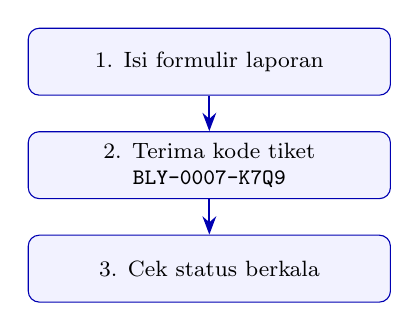
\begin{tikzpicture}[node distance=0.45cm]
  \node[alir] (p1) {1. Isi formulir laporan};
  \node[alir, below=of p1] (p2) {2. Terima kode tiket\\\texttt{BLY-0007-K7Q9}};
  \node[alir, below=of p2] (p3) {3. Cek status berkala};
  \draw[panah] (p1) -- (p2);
  \draw[panah] (p2) -- (p3);
\end{tikzpicture}
\hspace{0.8cm}
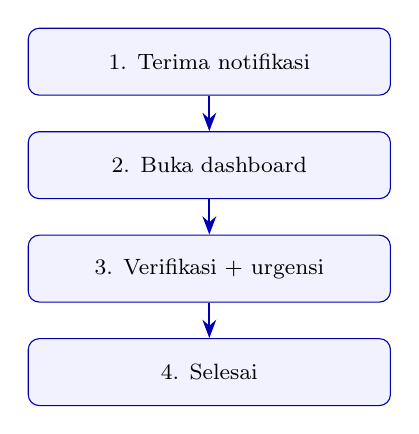
\begin{tikzpicture}[node distance=0.45cm]
  \node[alir] (a1) {1. Terima notifikasi};
  \node[alir, below=of a1] (a2) {2. Buka dashboard};
  \node[alir, below=of a2] (a3) {3. Verifikasi + urgensi};
  \node[alir, below=of a3] (a4) {4. Selesai};
  \draw[panah] (a1) -- (a2);
  \draw[panah] (a2) -- (a3);
  \draw[panah] (a3) -- (a4);
\end{tikzpicture}
\caption{Kiri: alur pelapor. Kanan: alur admin.}
\label{fig:alur}
\end{figure}

Kode tiket terdiri dari nomor urut dan kode acak, misalnya
\texttt{BLY-0007-K7Q9}, sehingga tidak dapat ditebak oleh pihak lain.

\section{Rincian Fitur}
\subsection{Untuk Siswa (Publik)}
\begin{itemize}[nosep]
  \item Formulir laporan: kategori, kronologi, waktu, lokasi, dan satu foto bukti.
  \item Kode tiket otomatis setiap laporan berhasil dikirim.
  \item Halaman cek status berupa linimasa: Diterima $\rightarrow$ Diverifikasi
        $\rightarrow$ Diproses $\rightarrow$ Selesai.
  \item Dapat dipasang sebagai aplikasi di HP (PWA) dari browser.
\end{itemize}
\subsection{Untuk Guru BK (Admin)}
\begin{itemize}[nosep]
  \item Login aman (sesi + password terenkripsi) dan fitur ganti password.
  \item Dashboard: saring berdasarkan status, cari berdasarkan kode tiket.
  \item Penentuan urgensi (Ringan, Sedang, Berat) dan ubah status laporan.
  \item Notifikasi ganda: lencana jumlah laporan baru + pesan Telegram otomatis.
\end{itemize}

\section{Panduan Penggunaan}
\subsection{Panduan Siswa}
\begin{enumerate}[nosep]
  \item Buka halaman utama, isi formulir sejujur-jujurnya, lampirkan foto bila ada.
  \item Tekan \textbf{Kirim Laporan}, lalu \textbf{simpan kode tiket} yang muncul
        (catat atau cetak halaman tersebut).
  \item Buka \textbf{Cek Tiket}, masukkan kode untuk melihat perkembangan status.
\end{enumerate}

\begin{figure}[h]
\centering
\fbox{\parbox{0.8\linewidth}{\centering \vspace{0.8cm}
\textit{[Screenshot: formulir laporan]} \\ \vspace{0.8cm}}}
\caption{Contoh tampilan formulir laporan.}
\end{figure}

\subsection{Panduan Guru BK}
\begin{enumerate}[nosep]
  \item Buka halaman admin, masuk dengan username dan password yang diberikan.
  \item Pantau lencana \textbf{baru} di dashboard; tiap laporan baru juga
        dikirim ke Telegram.
  \item Buka rincian laporan, tentukan urgensi, lalu majukan statusnya hingga
        \textbf{Selesai}.
  \item Segera ganti password bawaan melalui menu avatar di kanan atas.
\end{enumerate}

\textbf{Aktivasi notifikasi Telegram (5 menit):} (1) chat ke \texttt{@BotFather},
buat bot baru, salin token; (2) chat ke \texttt{@userinfobot} untuk melihat ID
chat; (3) kirim satu pesan ke bot baru tersebut; (4) serahkan token dan ID chat
kepada pengembang untuk dipasang.

\begin{figure}[h]
\centering
\fbox{\parbox{0.8\linewidth}{\centering \vspace{0.8cm}
\textit{[Screenshot: dashboard admin]} \\ \vspace{0.8cm}}}
\caption{Contoh tampilan dashboard admin.}
\end{figure}

\section{Ketentuan Serah Terima}
\begin{itemize}[nosep]
  \item Paket ini mencakup aplikasi versi 1.0 MVP sesuai rincian fitur di atas.
  \item Termasuk \textbf{satu kali revisi kecil} (teks, warna, tata letak).
  \item Fitur di luar daftar akan dibahas dan disepakati terpisah.
\end{itemize}

\appendix
\section{Arti Status dan Urgensi}
\begin{center}
\begin{tabular}{ll}
\toprule
\textbf{Status} & \textbf{Arti} \\
\midrule
Diterima & Laporan masuk, belum diperiksa \\
Diverifikasi & Laporan valid, siap ditindaklanjuti \\
Diproses & Sedang ditangani Guru BK \\
Selesai & Penanganan tuntas \\
\bottomrule
\end{tabular}
\qquad
\begin{tabular}{ll}
\toprule
\textbf{Urgensi} & \textbf{Arti} \\
\midrule
Ringan & Ditangani rutin \\
Sedang & Perlu perhatian khusus \\
Berat & Prioritas utama \\
\bottomrule
\end{tabular}
\end{center}

\section{Pertanyaan Umum}
\begin{enumerate}[nosep]
  \item \textbf{Apakah pelapor harus punya akun?} Tidak, pelaporan anonim.
  \item \textbf{Kode tiket hilang, bagaimana?} Hubungi Guru BK dengan menyebutkan
        waktu dan lokasi kejadian untuk penelusuran manual.
  \item \textbf{Apakah foto bukti wajib?} Tidak, tetapi sangat membantu verifikasi.
  \item \textbf{Siapa yang bisa melihat foto bukti?} Hanya admin yang sudah masuk.
\end{enumerate}

\end{document}
